Recall that linear PCA finds new components that reveal more information about the structure of high-dimensional data.
Since PCA is an orthogonal projection, the original data is rotated witin the original space of input variables.
The work of Sch\"olkopf, Smola, and M\"uller \cite{scholkopf1997kernel,scholkopf1998nonlinear} generalized PCA based on the successful application of kernel methods in support vector machines.
In kernel PCA, the inner product of the input space is replaced with the inner product of a feature space.
As such, the principal components of kernel PCA are nonlinear transformations of input variables, or features.

Using results from the previous section, a kernel function \(k\) defines a unique reproducing kernel Hilbert space \(H_k\) and feature map \(\Phi : X \to H_k\) such that
\begin{equation}
    \label{eqn:kernel-inner-product}
    k(x,y) = \langle \Phi(x), \Phi(y) \rangle,
\end{equation}
for all \(x, y \in H_k\).

\subsection{Covariance matrix and kernel matrix}
In PCA, we diagonalize \(X^\top X\).

\subsection{Centering in the feature space}
\label{sec:centering-in-the-feature-space}
Let \(\Phi : X \to H_k\) be a feature map determined by a kernel \(k\).
Since \(\Phi\) may be nonlinear, the image \(\Phi(x)\) of a centered vector \(x \in X\) is not guaranteed to be centered.
For an effective PCA algorithm, it is necessary to compute the kernel matrix of centered vectors in the feature space. \cite{scholkopf1998nonlinear}

Given \(x_1, \dots, x_n \in X\), the points
\begin{equation}
    \label{eqn:centered-features}
    \Phi_0(x_i) = \Phi(x_i) - \frac{1}{n} \sum_{i=1}^{n} \Phi(x_i), \quad \text{for \(i = 1,\dots,m\)}
\end{equation}
are the centered feature vectors in \(H_k\).
Then the centered kernel matrix becomes
\def\ipt#1{\left\langle #1 \right\rangle}
\begin{align*}
    [K_0]_{ij}
    &= \ipt{\Phi_0(x_i), \Phi_0(x_j)}\\
    &= \ipt{\Phi(x_i) - \frac{1}{n} \sum_{p=1}^{n} \Phi(x_p), \Phi(x_j) - \frac{1}{n} \sum_{q=1}^{n} \Phi(x_q)}\\
    &= \ipt{\Phi(x_i), \Phi(x_j)}
    \begin{aligned}[t]
        &- \frac{1}{n} \sum_{p=1}^{n} \ipt{\Phi(x_p), \Phi(x_j)}\\
        &- \frac{1}{n} \sum_{q=1}^{n} \ipt{\Phi(x_i), \Phi(x_q)}\\
        &+ \frac{1}{n^2} \sum_{p=1}^{n} \sum_{q=1}^{n} \ipt{\Phi(x_p), \Phi(x_q)}
    \end{aligned}\\
    % &= k(x_i, x_j) - \frac{1}{n} \sum_{p=1}^{n} k(x_p, x_j) - \frac{1}{n} \sum_{q=1}^{n} k(x_i, x_q) + \frac{1}{n^2} \sum_{p=1}^{n} \sum_{q=1}^{n} k(x_p, x_q)\\
    &= [K]_{ij} - \frac{1}{n} \sum_{p=1}^{n} [K]_{pj} - \frac{1}{n} \sum_{q=1}^{n} [K]_{iq} + \frac{1}{n^2} \sum_{p=1}^{n} \sum_{q=1}^{n} [K]_{pq},
\end{align*}
where \(K\) is the uncentered kernel matrix given by \([K]_{ij} = \ipt{\Phi(x_i), \Phi(x_j)}\).
% The term \(\frac{1}{n} \sum_{p=1}^{n} [K]_{pj}\) is the mean of the \(j\)-th column of \(K\), \(\frac{1}{n} \sum_{q=1}^{n} [K]_{iq}\) is the mean of the \(i\)-th row of \(K\), and \(\frac{1}{n^2} \sum_{p=1}^{n} \sum_{q=1}^{n} [K]_{pq}\) is the mean over all entries of \(K\).
Then the formula for the centered kernel matrix can be written as
\begin{equation}
    \label{eqn:centered-kernel-matrix}
    K_0 = K - \colmean(K) - \rowmean(K) + \mean(K).
\end{equation}
See notes in \Cref{subsec:matrix-operations,subsec:broadcasting}.
% \def\ones{\mathbf{1}_n}
% \begin{equation}
%     \label{eqn:centered-kernel-matrix}
%     K_0 = K - \ones K - K \ones + \ones K \ones,
% \end{equation}
% where \(\ones\) is the \(n \times n\) matrix whose entries are \(1/n\).
% So, the centered matrix \(K_0\) can be computed in terms of the kernel where \([K]_{ij} = k(x_i,x_j)\).

% \def\c{\mathbf{c}}
% \def\r{\mathbf{r}}
% For efficiency, the column means, row means, and entrywise mean of \(K\) can be precomputed and broadcast as \(m \times m\) arrays.
% Let
% \begin{align*}
%     \c &= \frac{1}{n} \begin{bmatrix}
%         \sum_{p=1}^{n} [K]_{p1}\\[4pt]
%         \sum_{p=1}^{n} [K]_{p2}\\[4pt]
%         \vdots\\[4pt]
%         \sum_{p=1}^{n} [K]_{pm}
%     \end{bmatrix}^\top,&
%     \r &= \frac{1}{n} \begin{bmatrix}
%         \sum_{q=1}^{n} [K]_{1q}\\[4pt]
%         \sum_{q=1}^{n} [K]_{2q}\\[4pt]
%         \vdots\\[4pt]
%         \sum_{q=1}^{n} [K]_{mq}
%     \end{bmatrix},&
%     \mu &= \frac{1}{n^2} \sum_{p=1}^{n} \sum_{q=1}^{n} [K]_{pq}.
% \end{align*}
% Then \Cref{eqn:centered-kernel-matrix} becomes
% \begin{equation}
%     \label{eqn:centered-kernel-computation}
%     K_0 = K - \c - \r + \mu,
% \end{equation}
% where \(\c\) is a \(1 \times m\) array broadcast to the rows of \(K\), \(\r\) is an \(m \times 1\) array broadcast to the columns of \(K\), and \(\mu\) is a scalar added to every entry of \(K\).

\begin{algorithm}
    \caption{Kernel PCA}
    \label{alg:kernel-pca}
    \KwIn{Data matrix \(A \in \RR^{n \times d}\), kernel function \(k\), number of components \(p \leq n\)}
    \KwOut{Transformed data \(\tilde{A} \in \RR^{n \times p}\)}
\end{algorithm}

\begin{example}
    Consider the problem of classifying points based on their radii.
    These points cannot be separated using a linear classifier in the two dimensions.
    However, by mapping them to a three-dimensional space, they can be separated by planes.
    Applying kernel PCA, these points can be sent to the RKHS associated with a Gaussian kernel without using an explicit feature map.
    The points in this high-dimensional feature space can then be projected onto the first three principal components to find separation boundaries.
    See \Cref{fig:gaussian-kpca-example}.
    \begin{figure}
        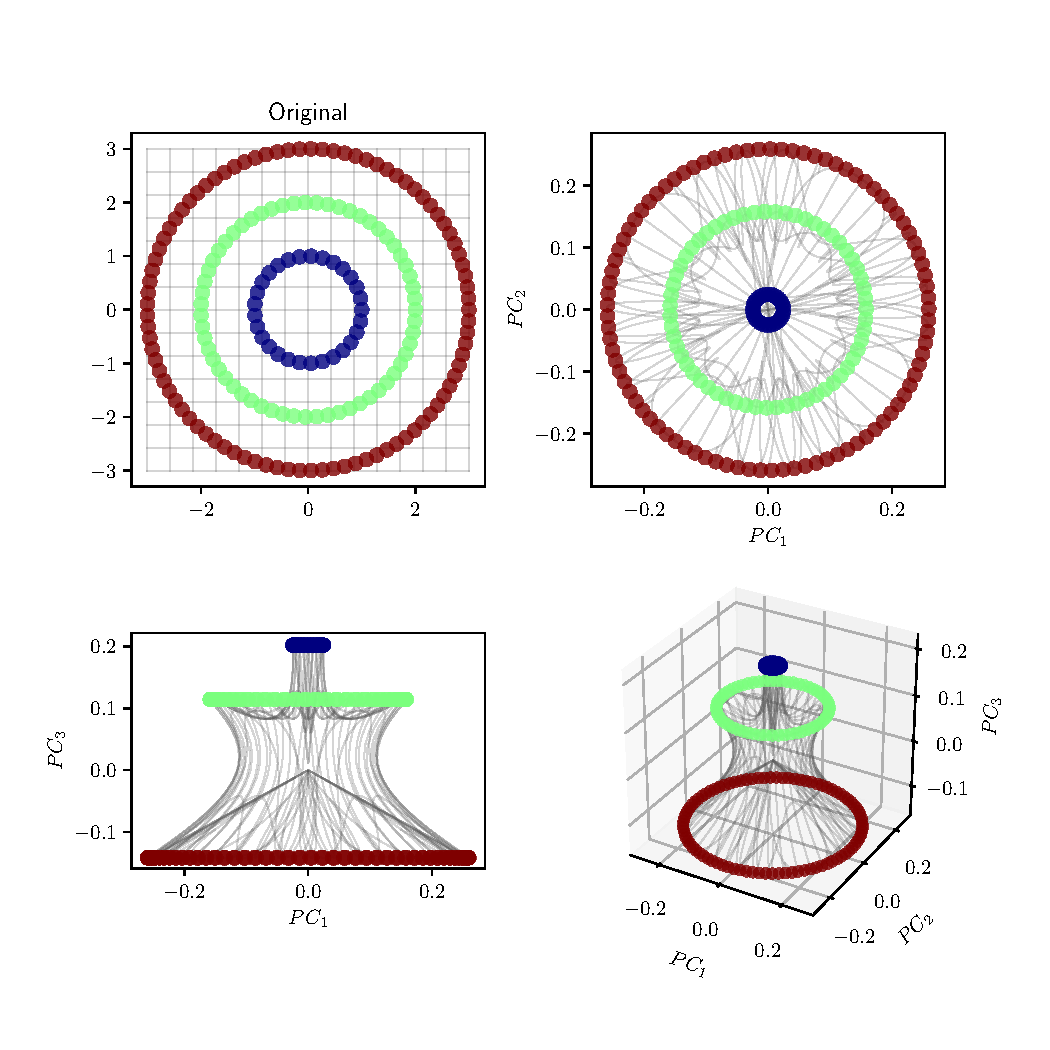
\includegraphics[width=\textwidth]{figs/fig_kpca_example.pdf}
        \caption{An idealized set of points in the plane are classified based on their radius. Kernel PCA with the Gaussian kernel is applied to find separation boundaries using the first three principal components.}
        \label{fig:gaussian-kpca-example}
    \end{figure}
\end{example}

% To do:
% - more about feature maps
% - use encode paper, kpca section for feature map/ feature space
% - nonlinear maps
% - rkhs
% - kpca algorithm
% - example